\vspace{-.5em}
\section{Are All Attention Heads Important?}
\label{sec:are_all_heads_important}

We perform a series of experiments in which we remove one or more attention heads from a given architecture at test time, and measure the performance difference. We first remove a single attention head at each time (\S\ref{sec:ablating_one}) and then remove every head in an entire layer except for one (\S\ref{sec:ablating_all_but_one}).
\vspace{-.5em}

% We then look at characteristics of those heads that cannot be removed without hurting performance significantly (\S\ref{sec:important_characteristics}).

% We perform a series of controlled experiments in which we remove one or more attention heads from a given architecture at test time, and measure the performance difference. We first remove a single attention head at each time (\S\ref{sec:ablating_one}), then remove every head in an entire layer except for one (\S\ref{sec:ablating_all_but_one}), and finally employ a heuristic method for pruning an arbitrary number of heads from the entire network (\S\ref{sec:pruning}).

\begin{figure*}[t!]
\begin{subfigure}[t]{0.48\textwidth}
\centering
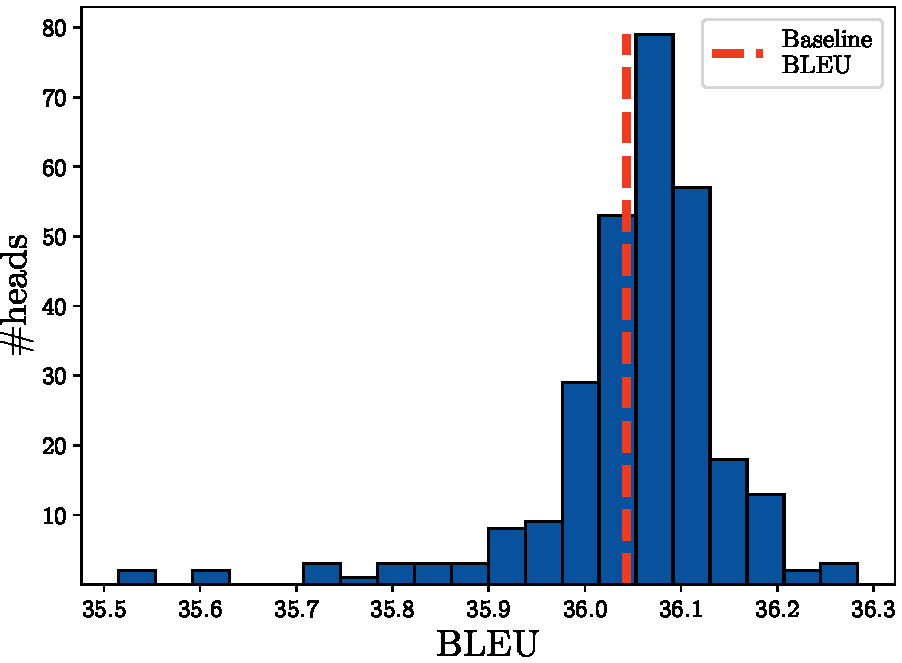
\includegraphics[width=\textwidth]{img/delta_distribs_wmt.pdf}
\caption{\label{fig:delta_distribs_wmt} \tfwmt{}
}
\end{subfigure}
~
\begin{subfigure}[t]{0.48\textwidth}
\centering
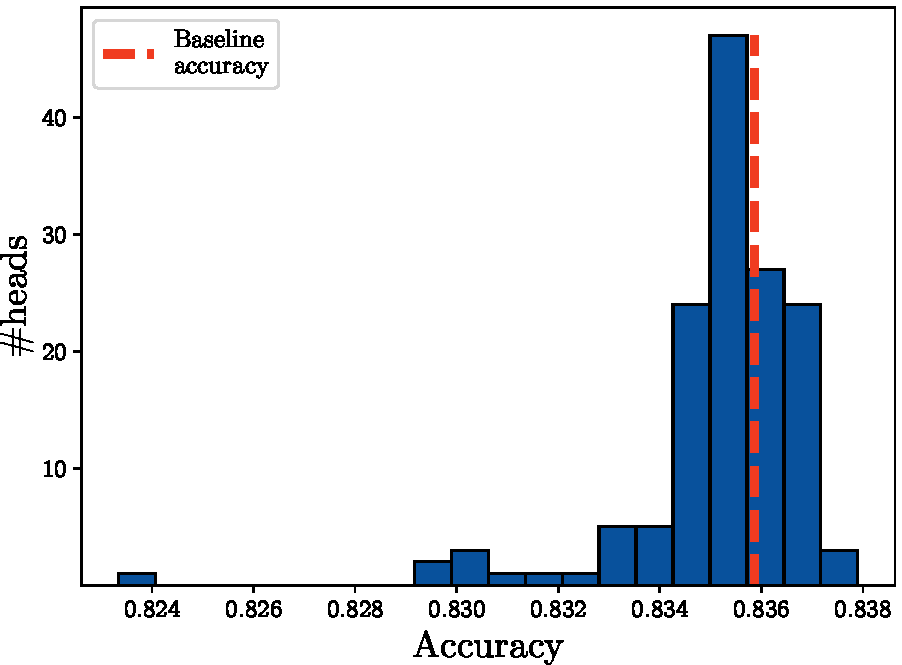
\includegraphics[width=\columnwidth]{img/delta_distribs_bert.pdf}
\caption{\label{fig:delta_distribs_bert} \bertmnli{}
}
\end{subfigure}
\caption{\label{fig:delta_distribs} Distribution of heads by model score after masking.}
\vspace{-1em}
\end{figure*}

\subsection{Experimental Setup}

In all following experiments, we consider two trained models:
% \gn{It might be worth pointing out what the difference between these two settings is. Specifically, these are important if they will affect our results later (e.g. Transformer-based MT has multiple attention mechanisms, while BERT only has one).}

\paragraph{\tfwmt{}} This is the original ``large'' transformer architecture from \citealt{vaswani2017attention} with 6 layers and 16 heads per layer, trained on the WMT2014 English to French corpus. We use the pretrained model of \citealt{ott2018scaling}.\footnote{\url{https://github.com/pytorch/fairseq/tree/master/examples/translation}} and report BLEU scores on the \texttt{newstest2013} test set. In accordance with \citealt{ott2018scaling}, we compute BLEU scores on the tokenized output of the model using Moses \citep{koehn2007moses}. Statistical significance is tested with paired bootstrap resampling \citep{koehn2004statistical} using \texttt{compare-mt}\footnote{\url{https://github.com/neulab/compare-mt}} \citep{neubig2019comparemt} with 1000 resamples. A particularity of this model is that it features 3 distinct attention mechanism: encoder self-attention (Enc-Enc), encoder-decoder attention (Enc-Dec) and decoder self-attention (Dec-Dec), all of which use \ac{mha}.

\paragraph{\bertmnli{}} BERT \citep{devlin2018bert} is a single transformer pre-trained on an unsupervised cloze-style ``masked language modeling task'' and then fine-tuned on specific tasks. At the time of its inception, it achieved state-of-the-art performance on a variety of \ac{nlp} tasks. We use the pre-trained \texttt{base-uncased} model of \citealt{devlin2018bert} with 12 layers and 12 attention heads which we fine-tune and evaluate on MultiNLI \citep{williams18multinli}. We report accuracies on the ``matched'' validation set. We test for statistical significance using the t-test. In contrast with the \tfwmt{} model, \bertmnli{} only features one attention mechanism (self-attention in each layer).
% 4 tasks from the GLUE Benchmark \citep{wang2018glue}: MNLI \citep{williams18multinli}, SST-2 \citep{socher2013recursive}, MRPC \citep{brocket2005automatically} and CoLA \citep{Warstadt2018NeuralNA}.

\subsection{Ablating One Head}
\label{sec:ablating_one}

% To understand the contribution of each individual head in a \ac{mha} based model $M$, we compute the difference in (task dependent) score $\mathcal{S}$ on dataset $X$ when the model is amputated of head $h$ in layer $l$: \omer{``amputated'' has very negative associations (war, traffic accidents, cancer). Use more neutral phrasings like "when head $h$ is removed from/ignored by the model".}
To understand the contribution of a particular attention head $h$, we evaluate the model's performance while masking that head (i.e. replacing $Att_h (x)$ with zeros). If the performance sans $h$ is significantly worse than the full model's, $h$ is obviously important; if the performance is comparable, $h$ is redundant given the rest of the model.

Figures \ref{fig:delta_distribs_wmt} and \ref{fig:delta_distribs_bert} shows the distribution of heads in term of the model's score after masking it, for \tfwmt{} and \bertmnli{} respectively. We observe that the majority of attention heads can be removed without deviating too much from the original score. Surprisingly, in some cases removing an attention head results in an increase in BLEU/accuracy.




To get a finer-grained view on these results we zoom in on the encoder self-attention layers of the \tfwmt{} model in Table \ref{tab:tfwmt_ablation}. Notably, we see that only 8 (out of 96) heads cause a statistically significant change in performance when they are removed from the model, half of which actually result in a higher BLEU score. This leads us to our first observation: \textbf{at test time, most heads are redundant given the rest of the model}.


\begin{table*}[t]
\centering
\setlength\tabcolsep{1.5pt}
\begin{tabular}{c|cccccccccccccccc}

\backslashbox{ Layer}{Head}& 1 & 2 & 3 & 4 & 5 & 6 & 7 & 8 & 9 & 10 & 11 & 12 & 13 & 14 & 15 & 16 \\
\hline\hline
1 & \small\color{NavyBlue} 0.03 & \small\color{NavyBlue} 0.07 & \small\color{NavyBlue} 0.05 & \small\color{Maroon} -0.06 & \small\color{NavyBlue} 0.03 & \small\color{Maroon} \underline{\bf -0.53} & \small\color{NavyBlue} 0.09 & \small\color{Maroon} \underline{\bf -0.33} & \small\color{NavyBlue} 0.06 & \small\color{NavyBlue} 0.03 & \small\color{NavyBlue} 0.11 & \small\color{NavyBlue} 0.04 & \small\color{NavyBlue} 0.01 & \small\color{Maroon} -0.04 & \small\color{NavyBlue} 0.04 & \small\color{NavyBlue} 0.00 \\
2 & \small\color{NavyBlue} 0.01 & \small\color{NavyBlue} 0.04 & \small\color{NavyBlue} 0.10 & \small\color{NavyBlue} \underline{\bf 0.20} & \small\color{NavyBlue} 0.06 & \small\color{NavyBlue} 0.03 & \small\color{NavyBlue} 0.00 & \small\color{NavyBlue} 0.09 & \small\color{NavyBlue} 0.10 & \small\color{NavyBlue} 0.04 & \small\color{NavyBlue} \underline{\bf 0.15} & \small\color{NavyBlue} 0.03 & \small\color{NavyBlue} 0.05 & \small\color{NavyBlue} 0.04 & \small\color{NavyBlue} 0.14 & \small\color{NavyBlue} 0.04 \\
3 & \small\color{NavyBlue} 0.05 & \small\color{Maroon} -0.01 & \small\color{NavyBlue} 0.08 & \small\color{NavyBlue} 0.09 & \small\color{NavyBlue} 0.11 & \small\color{NavyBlue} 0.02 & \small\color{NavyBlue} 0.03 & \small\color{NavyBlue} 0.03 & \small\color{NavyBlue} -0.00 & \small\color{NavyBlue} 0.13 & \small\color{NavyBlue} 0.09 & \small\color{NavyBlue} 0.09 & \small\color{Maroon} -0.11 & \small\color{NavyBlue} \underline{\bf 0.24} & \small\color{NavyBlue} 0.07 & \small\color{Maroon} -0.04 \\
4 & \small\color{Maroon} -0.02 & \small\color{NavyBlue} 0.03 & \small\color{NavyBlue} 0.13 & \small\color{NavyBlue} 0.06 & \small\color{Maroon} -0.05 & \small\color{NavyBlue} 0.13 & \small\color{NavyBlue} 0.14 & \small\color{NavyBlue} 0.05 & \small\color{NavyBlue} 0.02 & \small\color{NavyBlue} 0.14 & \small\color{NavyBlue} 0.05 & \small\color{NavyBlue} 0.06 & \small\color{NavyBlue} 0.03 & \small\color{Maroon} -0.06 & \small\color{Maroon} -0.10 & \small\color{Maroon} -0.06 \\
5 & \small\color{Maroon} \underline{\bf -0.31} & \small\color{Maroon} -0.11 & \small\color{Maroon} -0.04 & \small\color{NavyBlue} 0.12 & \small\color{NavyBlue} 0.10 & \small\color{NavyBlue} 0.02 & \small\color{NavyBlue} 0.09 & \small\color{NavyBlue} 0.08 & \small\color{NavyBlue} 0.04 & \small\color{NavyBlue} \underline{\bf 0.21} & \small\color{Maroon} -0.02 & \small\color{NavyBlue} 0.02 & \small\color{Maroon} -0.03 & \small\color{Maroon} -0.04 & \small\color{NavyBlue} 0.07 & \small\color{Maroon} -0.02 \\
6 & \small\color{NavyBlue} 0.06 & \small\color{NavyBlue} 0.07 & \small\color{Maroon} \underline{\bf -0.31} & \small\color{NavyBlue} 0.15 & \small\color{Maroon} -0.19 & \small\color{NavyBlue} 0.15 & \small\color{NavyBlue} 0.11 & \small\color{NavyBlue} 0.05 & \small\color{NavyBlue} 0.01 & \small\color{Maroon} -0.08 & \small\color{NavyBlue} 0.06 & \small\color{NavyBlue} 0.01 & \small\color{NavyBlue} 0.01 & \small\color{NavyBlue} 0.02 & \small\color{NavyBlue} 0.07 & \small\color{NavyBlue} 0.05 \\
\hline
\end{tabular}
\caption{\label{tab:tfwmt_ablation} Difference in BLEU score for each head of the encoder's self attention mechanism. Underlined numbers indicate that the change is statistically significant with $p<0.01$. The base BLEU score is $36.05$.
}
\end{table*}

\begin{table}[t!]
\begin{minipage}{0.45\textwidth}
\centering
\begin{tabular}{c|ccc}
Layer & Enc-Enc & Enc-Dec & Dec-Dec \\
\hline\hline
1 & \color{Maroon} \underline{\bf -1.31} & \color{NavyBlue} \underline{\bf 0.24} & \color{Maroon} -0.03 \\
2 & \color{Maroon} -0.16 & \color{NavyBlue} 0.06 & \color{NavyBlue} 0.12 \\
3 & \color{NavyBlue} 0.12 & \color{NavyBlue} 0.05 & \color{NavyBlue} 0.18 \\
4 & \color{Maroon} -0.15 & \color{Maroon} -0.24 & \color{NavyBlue} 0.17 \\
5 & \color{NavyBlue} 0.02 & \color{Maroon} \underline{\bf -1.55} & \color{Maroon} -0.04 \\
6 & \color{Maroon} \underline{\bf -0.36} & \color{Maroon} \underline{\bf -13.56} & \color{NavyBlue} 0.24 \\
\hline
\end{tabular}
\caption{\label{tab:tfwmt_ablation_all_but} Best delta BLEU by layer when only one head is kept in the \tfwmt{} model. Underlined numbers indicate that the change is statistically significant with $p<0.01$.}
\end{minipage}\hspace{1cm}
\begin{minipage}{0.45\textwidth}
\centering
\begin{tabular}{c|ccc|c}
Layer &  & & Layer &  \\
\hhline{==~==}
1 & \color{Maroon} -0.01\% & & 7 & \color{RoyalBlue} 0.05\% \\
2 & \color{RoyalBlue} 0.10\% & & 8 & \color{Maroon} -0.72\% \\
3 & \color{Maroon} -0.14\% & & 9 & \color{Maroon} -0.96\% \\
4 & \color{Maroon} -0.53\% & & 10 & \color{RoyalBlue} 0.07\% \\
5 & \color{Maroon} -0.29\% & & 11 & \color{Maroon} -0.19\% \\
6 & \color{Maroon} -0.52\% & & 12 & \color{Maroon} -0.12\% \\
\cline{1-2}\cline{4-5}
\end{tabular}
\caption{\label{tab:bertmnli_ablation_all_but} Best delta accuracy by layer when only one head is kept in the \bertmnli{} model. None of these results are statistically significant with $p<0.01$.}
\end{minipage}
\end{table}


\subsection{Ablating All Heads but One}
\label{sec:ablating_all_but_one}

% To go one step further and investigate whether multiple heads are indeed needed, 
This observation begets the question: is more than one head even needed? Therefore, we compute the difference in performance when all heads except one are removed, within a single layer. In Table \ref{tab:tfwmt_ablation_all_but} and Table \ref{tab:bertmnli_ablation_all_but} we report the best score for each layer in the model, i.e. the score when reducing the entire layer to the single most important head.

We find that, for most layers, one head is indeed sufficient at test time, even though the network was trained with 12 or 16 attention heads. This is remarkable because these layers can be reduced to single-headed attention with only $1/16$th (resp. $1/12$th) of the number of parameters of a vanilla attention layer.
However, some layers \emph{do} require multiple attention heads; for example, substituting the last layer in the encoder-decoder attention of \tfwmt{} with a single head degrades performance by at least 13.5 BLEU points.
We further analyze when different modeling components depend on more heads in \S\ref{sec:importance_per_part}.



Additionally, we verify that this result holds even when we don't have access to the evaluation set when selecting the head that is ``best on its own''. For this purpose, we select the best head for each layer on a validation set (\texttt{newstest2013} for \tfwmt{} and a 5,000-sized randomly selected subset of the training set of MNLI for \bertmnli{}) and evaluate the model's performance on a test set (\texttt{newstest2014} for \tfwmt{} and the MNLI-matched validation set for \bertmnli{}). We observe that similar findings hold: keeping only one head does not result in a statistically significant change in performance for 50\% (resp. 100\%) of layers of \tfwmt{} (resp. \bertmnli{}). The detailed results can be found in Appendix \ref{sec:ablating_all_but_one_add}.



\subsection{Are Important Heads the Same Across Datasets?}
\label{sec:across_datasets}

There is a caveat to our two previous experiments: these results are only valid on specific (and rather small) test sets, casting doubt on their generalizability to other datasets. As a first step to understand whether some heads are universally important, we perform the same ablation study on a second, out-of-domain test set. Specifically, we consider the MNLI ``mismatched'' validation set for \bertmnli{} and the MTNT English to French test set \citep{michel-neubig-2018-mtnt} for the \tfwmt{} model, both of which have been assembled for the very purpose of providing contrastive, out-of-domain test suites for their respective tasks.

We perform the same ablation study as \S\ref{sec:ablating_one} on each of these datasets and report results in Figures \ref{fig:correl_bleu} and \ref{fig:correl_acc}. We notice that there is a positive, $>0.5$ correlation ($p<001$) between the effect of removing a head on both datasets. Moreover, heads that have the highest effect on performance on one domain tend to have the same effect on the other, which suggests that the most important heads from \S\ref{sec:ablating_one} are indeed ``universally'' important.

\begin{figure*}[t!]
\begin{subfigure}[b]{0.47\textwidth}
\centering
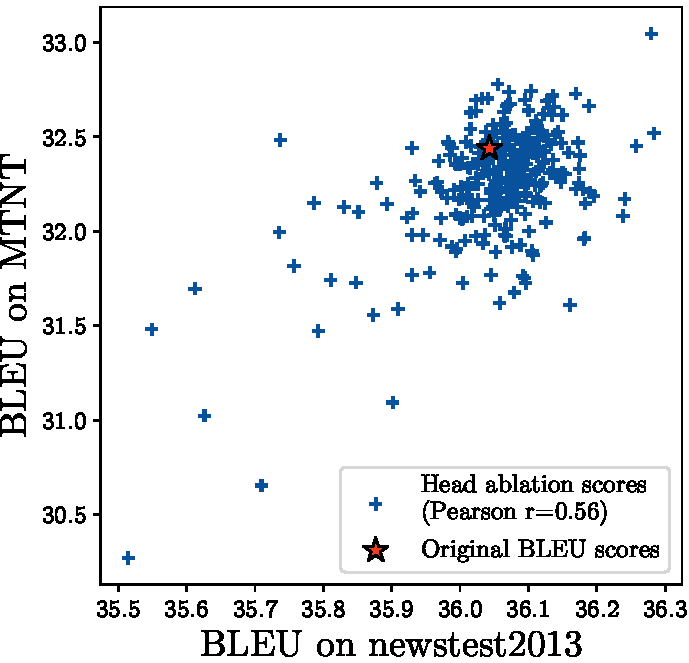
\includegraphics[width=\textwidth]{img/correl_bleu.pdf}
\caption{\label{fig:correl_bleu} BLEU on \texttt{newstest2013} and MTNT when individual heads are removed from \tfwmt{}. Note that the ranges are not the same one the X and Y axis as there seems to be much more variation on MTNT.
}
\end{subfigure}
~
\begin{subfigure}[b]{0.48\textwidth}
\centering
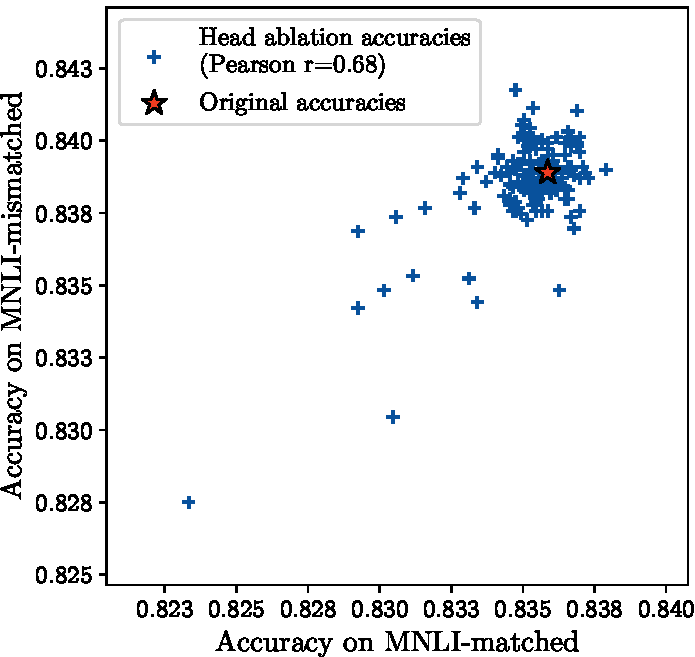
\includegraphics[width=\columnwidth]{img/correl_acc.pdf}
\caption{\label{fig:correl_acc} Accuracies on MNLI-matched and -mismatched when individual heads are removed from \bertmnli{}. Here the scores remain in the same approximate range of values.
}
\end{subfigure}
\caption{Cross-task analysis of effect of pruning on accuracy}
\end{figure*}